%!TEX root=../../main.tex


\subsubsection{Single-Source Shortest-Paths}
In this section, we compare the different frameworks in their performance on the SSSP algorithm. We first analyze the frameworks on a single computation node and compare to the distributed setup after that.
\paragraph{Single-node}
\begin{figure*}
	\begin{subfigure}{0.32\textwidth}
		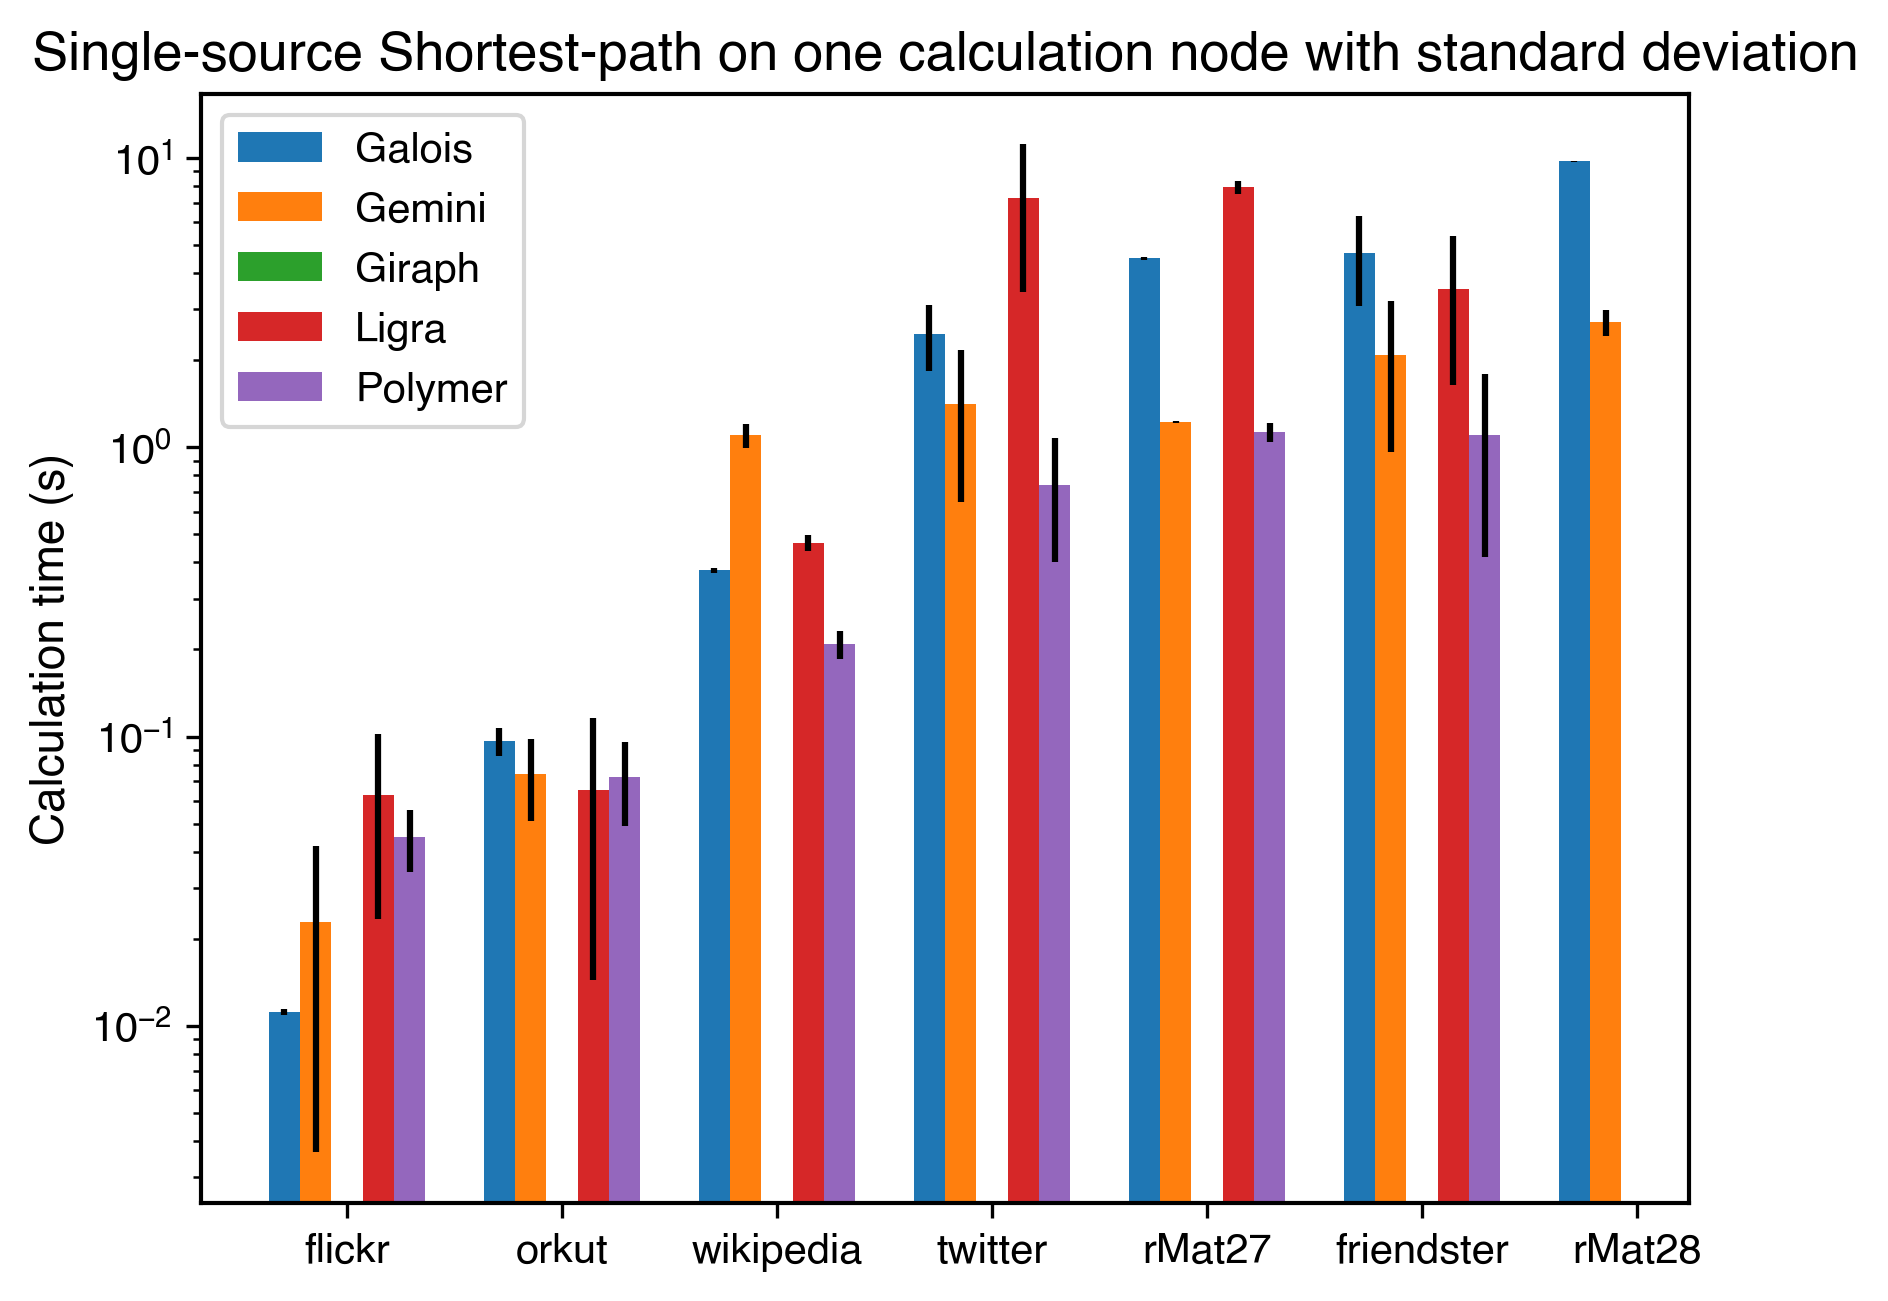
\includegraphics[width=\linewidth]{../../plots/singleNodeSSSP_calcTime.png}
		\caption{Calculation times}
		\label{fig:singleNodeSSSP_calc}
	\end{subfigure}
	\hfil
	\begin{subfigure}{0.32\textwidth}
		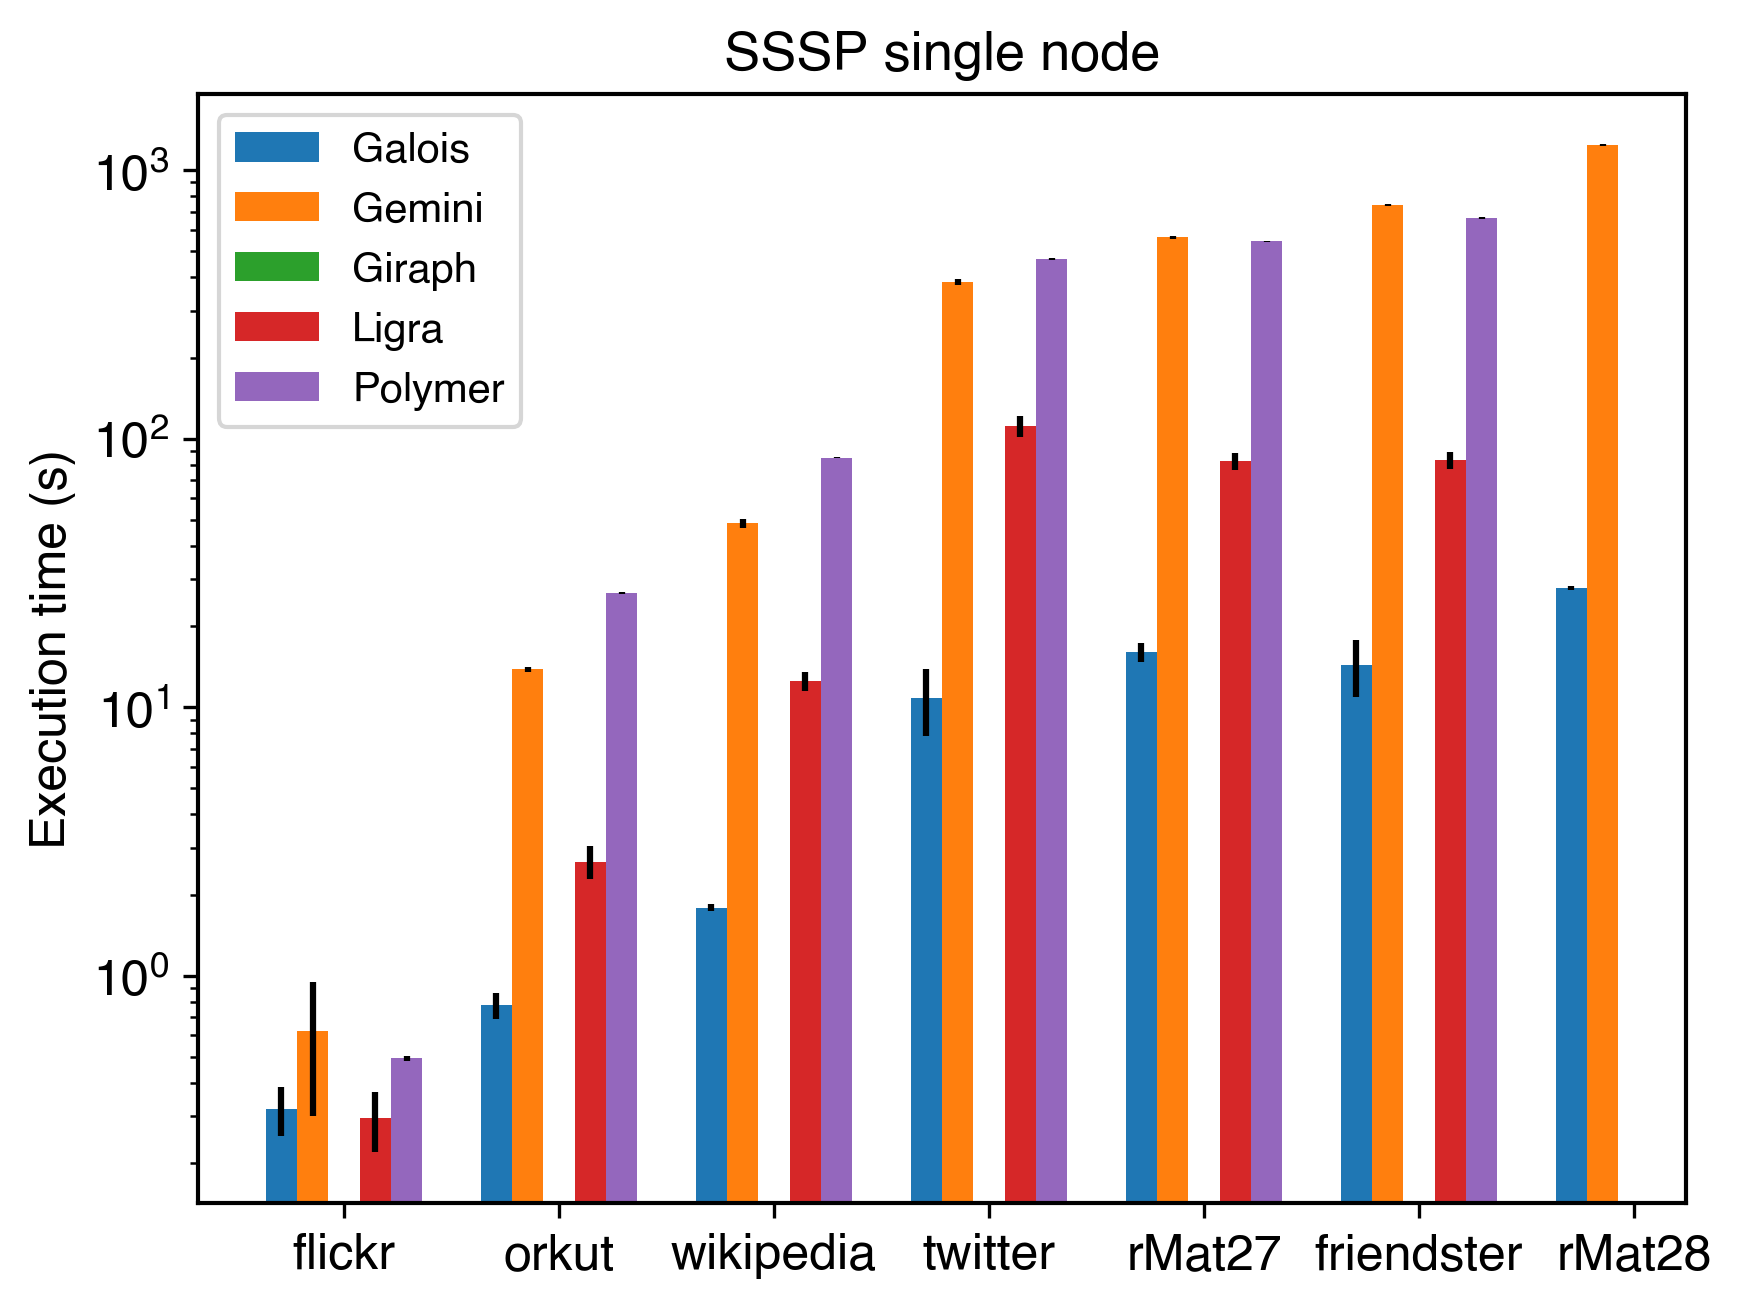
\includegraphics[width=\linewidth]{../../plots/singleNodeSSSP_execTime.png}
		\caption{Execution times}
		\label{fig:singleNodeSSSP_exec}
	\end{subfigure}
	\hfil
	\begin{subfigure}{0.32\textwidth}
		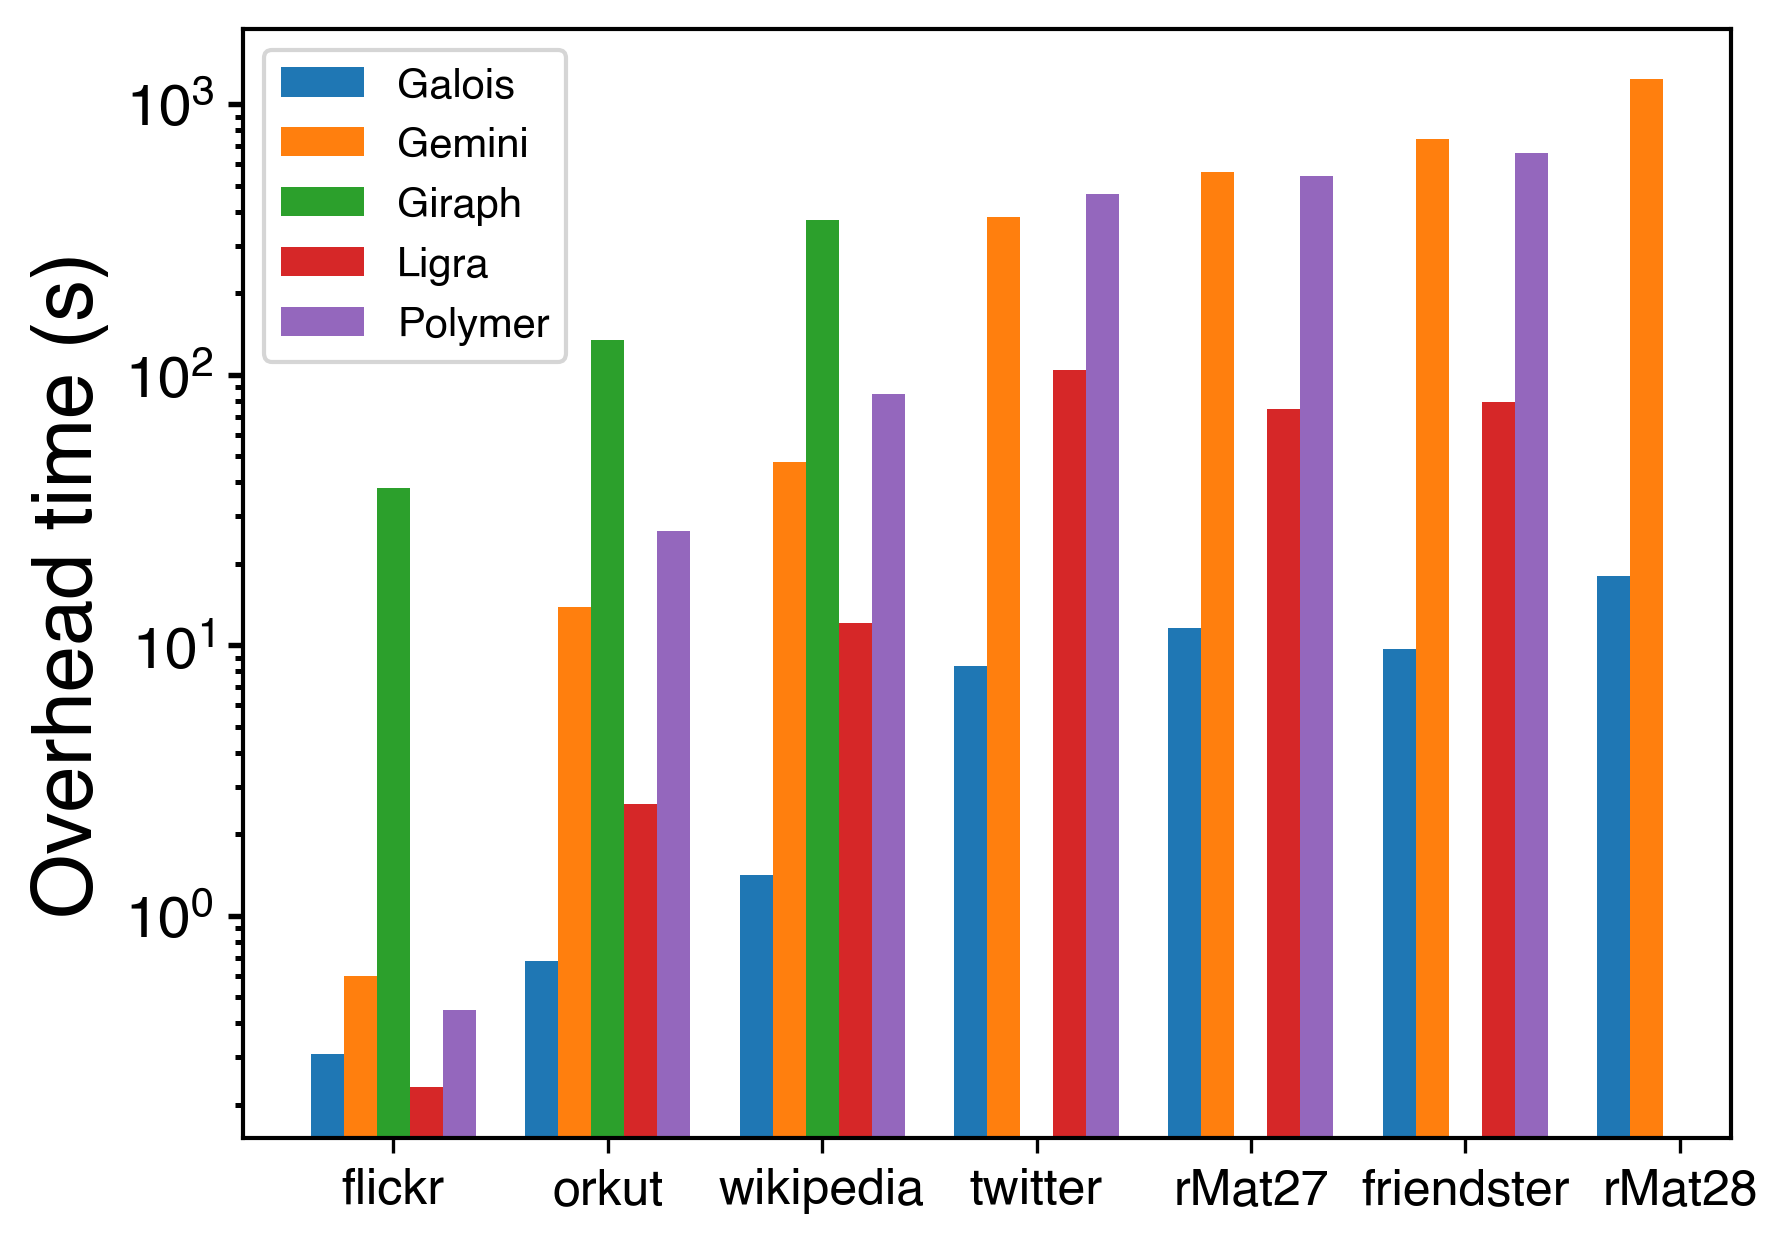
\includegraphics[width=\linewidth]{../../plots/singleNodeSSSP_overheadTime.png}
		\caption{Overhead time}
		\label{fig:singleNodeSSSP_overhead}
	\end{subfigure}
	\caption{Average times for SSSP on a single computation node, black bars represent one standard deviation in our testing.}
	\label{fig:singleNodeSSSP}
\end{figure*}
Beginning with the single-node performance, \autoref{fig:singleNodeSSSP} shows the average calculation and execution times for SSSP on the different frameworks.
Note, that Giraph ran out of memory ($>$250 GB) for all graphs larger than wikipedia (twitter, rMat27, friendster and rMat28). Thus, the data points on the larger graphs for Giraph are missing in the figures and our evaluation. 
Also, both Ligra and Polymer failed on rMat28.

Upon analyzing the calculation time (cf. \autoref{fig:singleNodeSSSP_calc}), most obvious is the fact that Giraph is at least one order of magnitude slower than any other framework. The only exception is Gemini, where Giraph is \emph{only} 4$\times$ slower on wikipedia. In general however, Giraph is on average 24$\times$ slower than the other frameworks on flickr, 17$\times$ on orkut and 12$\times$ on wikipedia.

Comparing the other frameworks (i.e. excluding Giraph in the further comparisons), shows them to perform similar on the smaller graphs. There, the average calculation times of the four frameworks (Galois, Gemini, Ligra, Polymer) are 35ms on flickr, 77ms on orkut and 538ms on wikipedia. 
The four frameworks are close to this average for the smaller graphs. Galois and Gemini being 24ms and 12ms faster than the average. Ligra and Polymer are slower by 27ms and 9ms.
Orkut is the graph where all the four frameworks are within 20ms of their average, Galois being the outlier at 19ms slower than average.
For wikipedia, Galois and Ligra are close to each other, while Gemini is 560ms (104\%) slower than the average of the four frameworks.
And Polymer is the fastest framework on wikipedia, being 330ms (61\%) faster than the others.
For the larger graphs, Polymer has the shortest computation time as well. Gemini is second, taking about 1.9$\times$ times the computation time of Polymer on twitter and friendster while being equally fast (8\% longer) on rMat27. Galois and Ligra however have much longer computation times compared to Polymer. Galois takes anywhere from 3.3$\times$ (twitter) to 4.2$\times$ (friendster) the computation time of Polymer.
Ligra requires between 3.2$\times$ (friendster) and 9.8$\times$ (twitter) the computation time of Polymer on the larger graphs. This makes Ligra the slowest Framework on both twitter and rMat27. Galois is the slowest on friendster.
However, while especially Galois is comparably slow to Polymer in the computation time, it is important to keep in mind that Polymer could not finish computation on rMat28. Meanwhile both Gemini and Galois managed just fine.

The execution times show Galois to be the clear winner on most graphs (cf. \autoref{fig:singleNodeBFS_exec}).
It has the smallest computation times on all graphs except flickr, where Galois is 25ms (8\%) slower than Ligra. 
On the other 5 graphs however, Galois has the smaller execution time by one or sometimes even two orders of magnitude. 
For example, on orkut Galois requires 0.78s to execute, while the other frameworks require between 2.66s (Ligra) and 26.6s (Polymer).
This goes on for the larger graphs, Ligra being second-fastest. Polymer and Gemini close together but both always at least one order of magnitude slower than Galois.

\paragraph{Distributed}
\begin{figure*}
	\centering
	\begin{subfigure}{0.32\textwidth}
		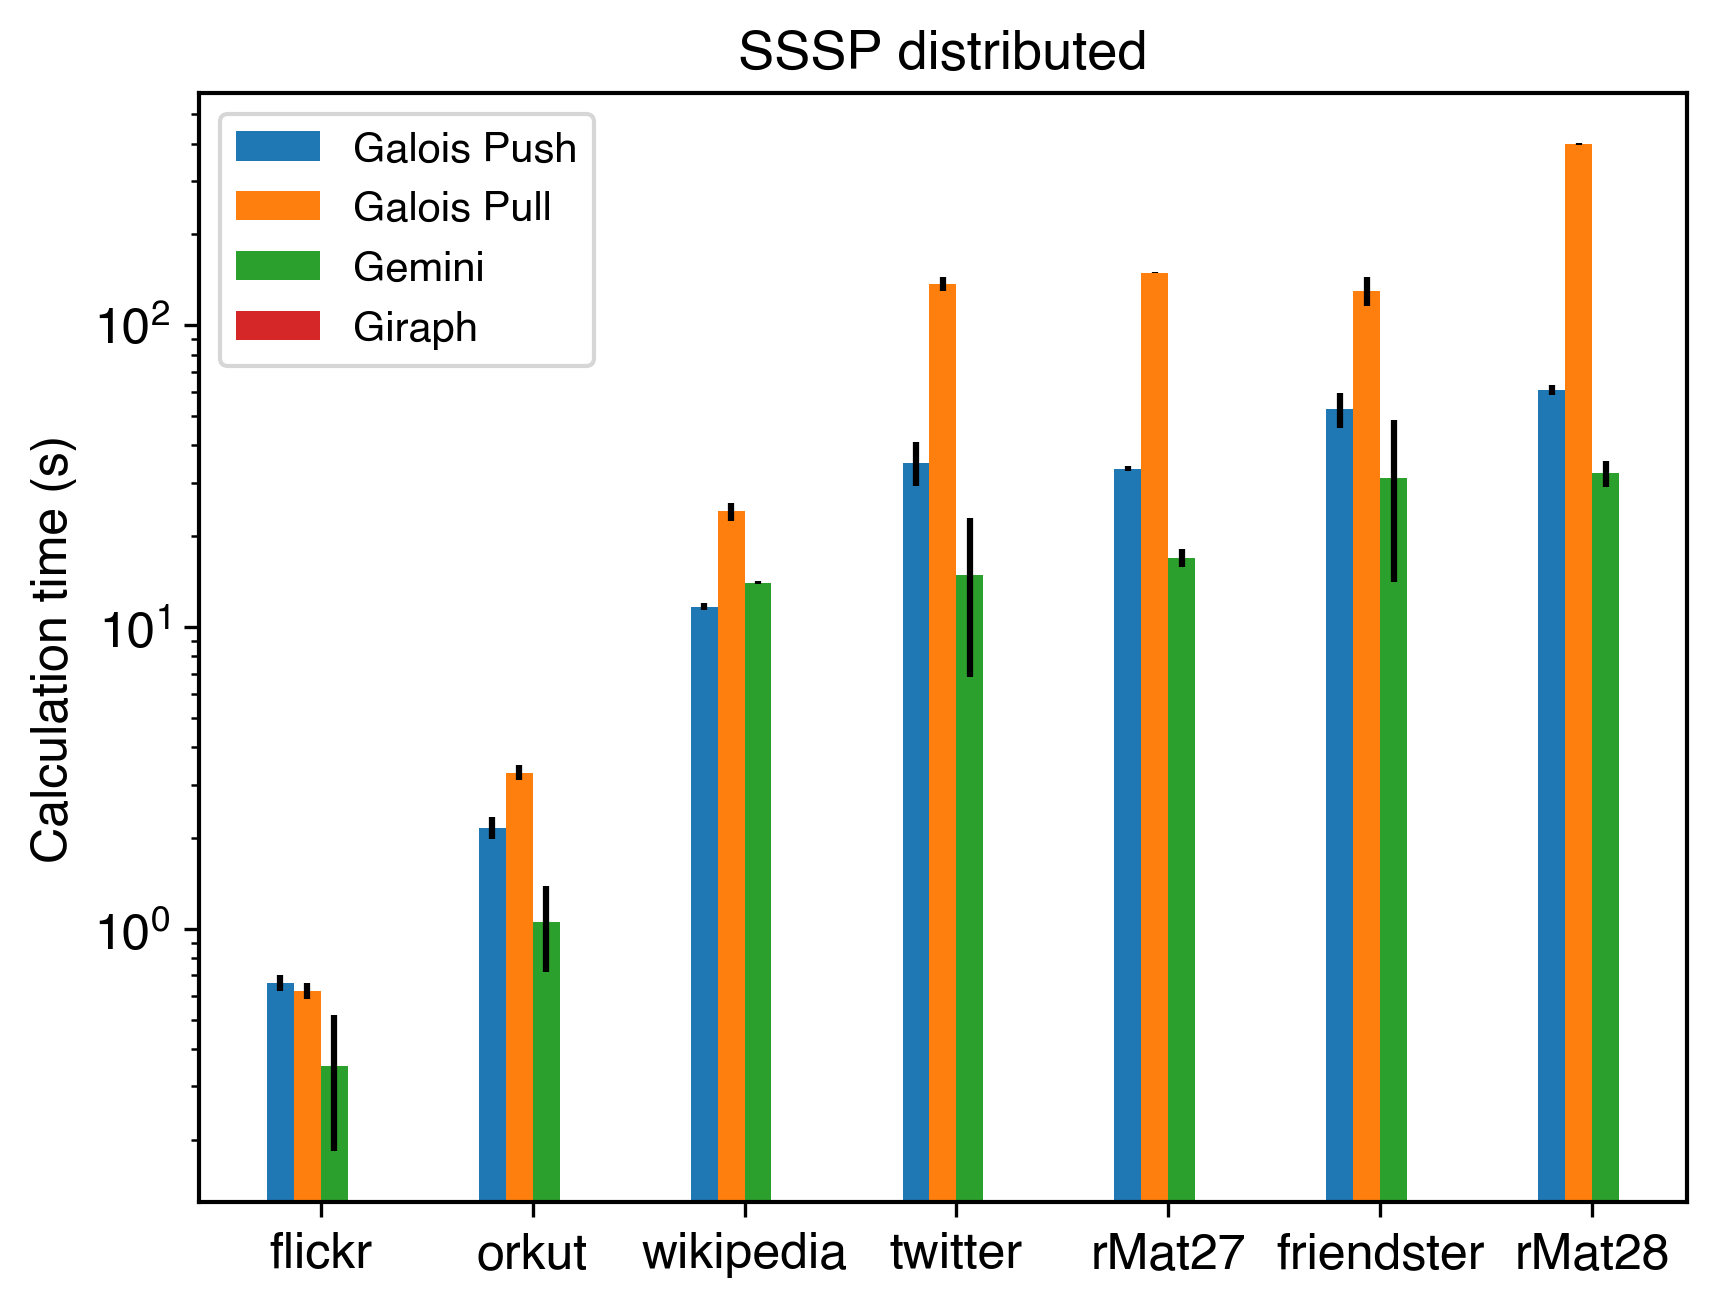
\includegraphics[width=\linewidth]{../../plots/distributedSSSP_calcTime.png}
		\caption{Calculation times}
		\label{fig:distributedSSSP_calc}
	\end{subfigure}
	\hfil
	\begin{subfigure}{0.32\textwidth}
		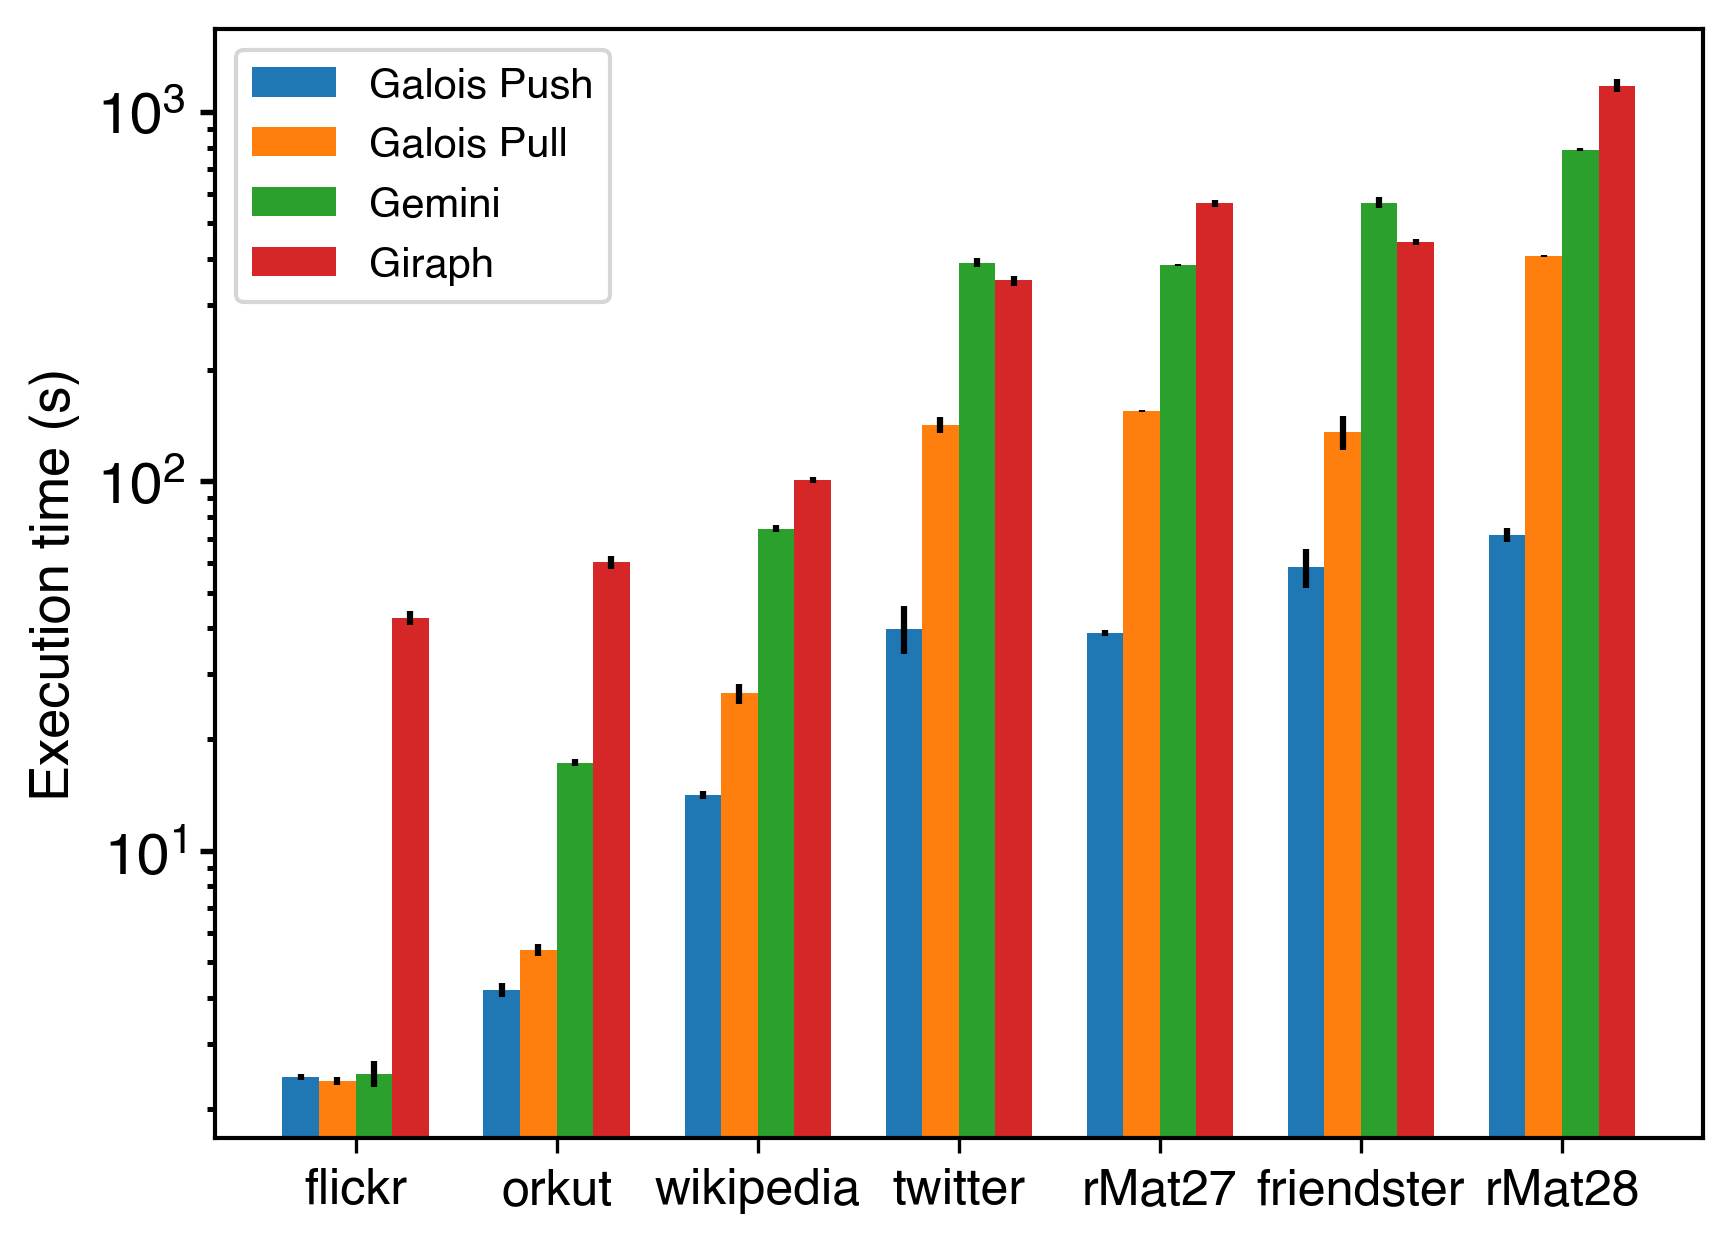
\includegraphics[width=\linewidth]{../../plots/distributedSSSP_execTime.png}
		\caption{Execution times}
		\label{fig:distributedSSSP_exec}
	\end{subfigure}
	\hfil
	\begin{subfigure}{0.32\textwidth}
		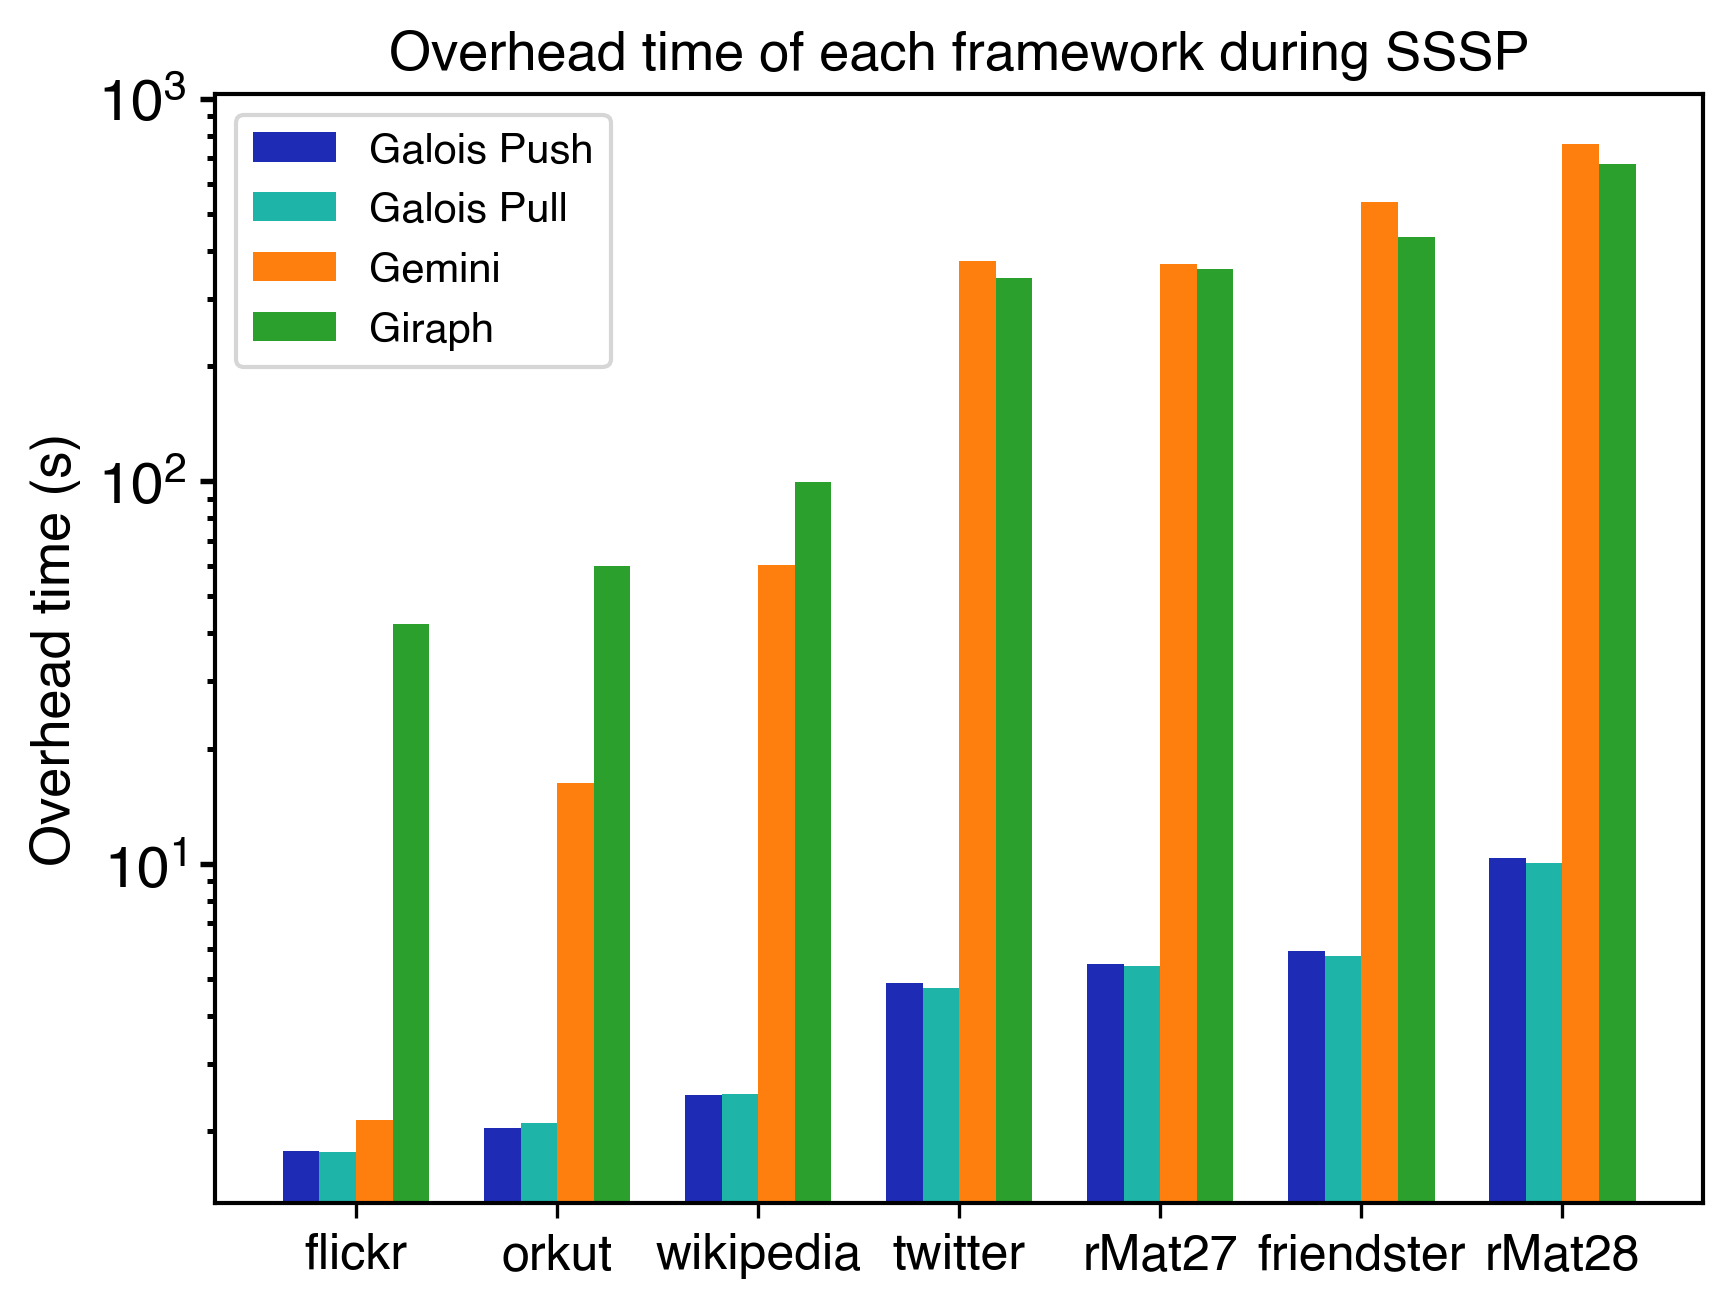
\includegraphics[width=\linewidth]{../../plots/distributedSSSP_overheadTime.png}
		\caption{Overhead times}
		\label{fig:distributedSSSP_overhead}
	\end{subfigure}
	\caption{Average times for SSSP on the distributed cluster, black bars represent one standard deviation in our testing.}
	\label{fig:distributedSSSP}
\end{figure*}
On the distributed cluster, we find similar results as on the single node (cf. \autoref{fig:distributedSSSP}).
Both Galois implementations have significantly smaller execution times compared to Gemini or Giraph on all graphs (cf. \autoref{tbl:ssspexec}).
You can see Gemini being worse by at least a factor of 4 compared to Galois Push on all graphs except flickr.
Giraph's execution times in comparison to this are even worse, taking at least 7$\times$ longer than Galois Push on all graphs.
Comparing the two Galois implementations, we find the calculation and execution times to be similar on smaller graphs and Push being the superior implementation for SSSP on larger data sets. Galois Pull is anywhere from just as fast to 3.5$\times$ slower on real-world data sets compared to the Push variant. The synthetic graphs are more extreme. Execution times are close to 4$\times$ (rMat27) and 5$\times$ (rMat28) longer on Pull.
Evidently, Galois Push is the fastest algorithm in our lineup on 6 out of 7 graphs. With the exception being flickr, where Galois Push takes negligibly longer than the Pull counterpart.


\begin{table}
\renewcommand{\arraystretch}{1.2}
\tiny
\centering
\caption{Distributed SSSP Execution Times and Their Realation to Galois Push}
\begin{tabular}{crrrrrrrr}
\toprule
\bf{Data Set}&
\multicolumn{2}{c}{\bf Galois Push}&\multicolumn{2}{c}{\bf Galois Pull}&\multicolumn{2}{c}{\bf Gemini}&\multicolumn{2}{c}{\bf Giraph}\\
&$\times$&(s)&$\times$&(s)&$\times$&(s)&$\times$&(s)\\\midrule
flickr & 1.0 & (2.4) & 0.97 & (2.4) & 1.02 & (2.5) & 17.46 & (42.6)\\
orkut & 1.0 & (4.2) & 1.28 & (5.4) & 4.12 & (17.3) & 14.38 & (60.4)\\
wikipedia & 1.0 & (14.2) & 1.88 & (26.6) & 5.26 & (74.5) & 7.11 & (100.8) \\
twitter & 1.0 & (40.0) & 3.56 & (142.2) & 9.79 & (391.1) & 8.76 & (349.9)\\
rMat27 & 1.0 & (39.0) & 3.98 & (154.9) & 9.91 & (386.0) & 14.52 & (565.8)\\
friendster & 1.0 & (58.5) & 2.32 & (136.0) & 9.72 & (568.9) & 7.59 & (444.0)\\
rMat28 & 1.0 & (71.5) & 5.7 & (407.9) & 11.07 & (792.0) & 16.5 & (1180.2)\\\bottomrule
\end{tabular}
\label{tbl:ssspexec}
\end{table}

When taking a closer look at Giraph, it seems to not cope well with synthetic data sets. Analyzing the computation times in \autoref{fig:distributedSSSP_calc}, we see that it is the fastest framework on our real-world graphs. And that with a considerable margin of other frameworks always taking at least 50\% longer (lower bound here is Gemini on flickr) up to Galois Pull needing 18$\times$ more time on wikipedia.
On both synthetic graphs however, Giraph is actually the slowest to compute. Giraph requires 12$\times$ or even 15$\times$ the computation time of Gemini on rMat27 or rMat28 respectively.
While Giraph's computation times are very competitive, when comparing the execution times in \autoref{fig:distributedSSSP_exec} we see that Giraph is actually the slowest framework on 5 out of 7 graphs. For the other two, namely twitter and friendster, Giraph is second slowest with only Gemini taking longer to complete.
Giraph and Gemini's very long execution times are only due to their overhead being many orders of magnitude larger than Galois overhead (\autoref{fig:distributedSSSP_overhead}).
Overhead for Gemini is greater than that of Galois on every graph. From just a 20\% increase on flickr up to friendster, where the overhead is 90$\times$ that of Galois Push.
For Giraph the overhead times are not as extreme but still generally worse. Even on flickr, Giraph's overhead time is already 23$\times$ that of Galois. On friendster, where Gemini was worst, Giraph \emph{only} requires 73$\times$ the overhead time of Galois.

